\input{preambletalk}
\title[An approach to MSO-transductions]{An algebraic approach to equivalence of MSO-definable graph transductions}

\author[Schmude, J.]{
	Boja{\'n}czyk, M.\inst{1}, \underline{Schmude, J.\inst{1}} }

\institute[University of Warsaw]{\inst{1}University of Warsaw %\and \inst{2} University of XXX
}

\date[18 February 2020]{S{\'e}minaire de l'{\'e}quipe M{\'e}thodes Formelles \\LaBRI\\18 February 2020}
\begin{document}
%\iffalse
\begin{frame}%slajd tytulowy
	\titlepage 
\end{frame}	
\begin{frame}{Main theorem}
%	Joint work with Miko{\l{}}aj Boja{\'n}czyk.\\
	Our main result (ongoing work):
	\begin{tw}The following problem is decidable:\\
		\underline{Input:}
		$$
		\xymatrix{
			\parbox{2cm}{
				graphs of \\ treewidth k}	\ar[r] ^{f, g}_{mso_2} &	\parbox{2cm}{
				graphs of \\ treewidth k}	
		}
		$$
		
		\underline{Question:} Are $f,g$ $\sim$-equivalent:
		
		$$
			\forall G \in \text{treewidth } k: \quad f(G) \sim g(G),
		$$
		
		$\sim$: equivalence relation (not isomorphism), defined later.
	\end{tw}
\pause
"$\sim$" $=$ "isomorphism" $\Ra$ equivalence problem.
\end{frame}

%\iffalse
\section{Overview}
\begin{frame}{MSO$_2$-definable transductions}
\textbf{MSO$_2$ transductions } -- nondeterministic (this talk: \underline{functional}) graph transformations, described by MSO$_2$ formulas (quantify over both vertices and edges).
\\
In particular, \textbf{linear size increase}, where $|G| = |V| + |E|$.
\pause
\\
\textbf{examples:} 
\pause
\begin{itemize}
	\item delete edges belonging only to nonsimple paths from $s$ to $t$.
	\item cycle $\mapsto$ path, same number of vertices (\underline{nondeterministic functional}).
\end{itemize}
\pause
\textbf{nonexamples:} \textcolor{blue}{MSO$_1$} but not MSO$_2$-definable:
\begin{itemize}
	\item neighbour of a neighbour \textcolor{blue}{($E'(x,y) = \exists z\ E(x, z) \wedge E(z, y).$)}
	\item $G \mapsto \text{ clique of size } |V(G)|$ \textcolor{blue}{($E'(x,y) = \top$)}
\end{itemize}
\end{frame}
\begin{frame}{Graph of treewidth $k$}
graph of treewidth $k$ 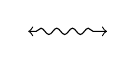
\begin{tikzpicture}
\draw [<->,decorate,decoration={snake,amplitude=.4mm,segment length=2mm,post length=1mm, pre length=1mm}]
(0,0) -- (1,0);
\end{tikzpicture} tree decomposition of width $k+1$.
\pause
\\
\textbf{examples:}
\\
\pause
graph of treewidth 1 = tree \\ \pause
\begin{tikzpicture}\def\nhing{0.75}
\node (1) at (0, 0) {1};
\node (2) at (1,\nhing) {2};
\node (3) at (1,-\nhing) {3};
\node (4) at (2,\nhing + 0.25) {4};
\node (5) at (3,\nhing) {5};
\node (6) at (3,-\nhing) {6};
\node[circle] (7) at (4,0) {7};
%
\draw (1) -- (2); \draw (1) -- (3); \draw (2) -- (3); \draw (2) -- (4); \draw (2) -- (5); \draw (4) -- (5); \draw (3) -- (6); \draw (5) -- (6); \draw (5) -- (7); \draw (6) -- (7); 
%
\pause
%
\node[ellipse, draw=black] (123) at (7,0) {123};
\node[ellipse, draw=black] (236) at (8.5,0) {236};
\node[ellipse, draw=black] (245) at (10,\nhing) {245};
\node[ellipse, draw=black] (567) at (10,-\nhing) {567};
%
\draw[-] (123) -- (236); \draw (236) -- (245); \draw (236) -- (567); 
\draw[|->] (7) -- (6.15, 0) node[midway, yshift=0.125cm] (labelka) {\tiny{tree decomposition}};
\node[below of= labelka, yshift = 0.75cm] (labelka dolna) {\tiny{of width 3}};
\end{tikzpicture}

\onslide<6->
{
\begin{tw}[Seese, '91]\def\C{\ens{\mathcal{C}}} \def\D{\ens{\mathcal{D}}}
	Let \C, \D be a classes of graphs. If equivalence is decidable for \C -to-\D MSO$_2$ transductions, then $\C, \D \subset graphs\ of\ treewidth\ k$, for some $k>0$.
\end{tw}
}
%Image tw=k ma ograniczony treewidth? TAK, Courcelle 07
\end{frame}
\begin{frame}{The equivalence relation $\sim$}
\begin{tw}[ICALP'18, Dell, Grohe, Rattan]
	For all graphs $G$ and $H$, the following are equivalent: 
	\begin{enumerate}[(i)]
		\item \only<4>{\textcolor{blue}{number of length-$n$ walks on $G$ and $H$ are equal, for all $n \geq 0$,}}
		\item
		there is a square matrix $X$ with real values, possibly negative:
			\begin{center}
				$A_GX = XA_H, \quad \textcolor{grey}{\text{$A_G$ -- adjacency matrix}}$\\
				\hspace{-1.6cm}\text{each row of } X \text{ sums up to 1}\\
				\hspace{-1.1cm}\text{each column of } X \text{ sums up to 1}
			\end{center}
		\pause
		%\begin{uw}
		 \textbf{remark}\\
		\ldots nonnegative integer-valued $X$ \ldots $\Lra$ $G, H$ are isomorphic.\\
		\pause
		\ldots nonnegative real-valued $X$ \ldots  $\Lra$ $G, H$ are fractionally isomorphic.
		%\end{uw}
		\pause
	\end{enumerate}
\end{tw}
\end{frame}
\begin{frame}{Overview}
\begin{tw}[Boja{\'n}czyk, S., '19] The following problem is decidable:\\
	\underline{Input:}
	$$
	\xymatrix{
		\parbox{2cm}{
		graphs of \\ treewidth k}	\ar[r] ^{f, g}_{mso} &	\parbox{2cm}{
		graphs of \\ treewidth k}	
	}
	$$
	
	\underline{Question:} Are $f,g$ equivalent:
	
	$\forall G \in \text{treewidth } k \quad f(G) \sim g(G)$,
	
	$\sim$: \textcolor{blue}{number of length-$n$ walks on $G$ and $H$ are equal, for all $n \geq 0$}
\end{tw}
\pause
We build on two following theorems.\\
\pause
\begin{itemize}
	\item 
%\begin{tw}
	$\lbrack$ '12, Seidl et al. $\rbrack$ Equivalence is decidable for tree-to-\Q register transducers. (can replace \Q with \Q(X) or power series) \pause \\
	% (ACKERMANN-hard)
	%polynomial automata
	%(\textcolor{blue}{extends to other rings, e.g. $\Z[X], \Q(X)$, \ldots })
	\item
	tree-to-treewidth $k$ MSO-transductions = \textcolor{blue}{ register transducers over $(k+1)$-sourced graph algebra.} (works also for treewidth $k$-to-treewidth $k$)
%\end{tw}
\end{itemize}
\end{frame}


\begin{frame}{Register transducers over algebra \A}
Let \A be an algebra, e.g. $(\Q, +, \cdot), (\{a, b\}^*, \cdot)$, %\parbox{
($k$-sourced graphs, "Courcelle" operations)
%}
.\\
\textbf{string-to-\A register transducers} Syntax: $DFA\ + $ registers that store \A. Example: \A = $(\Q, +, \cdot)$.\\
\begin{itemize}
	\item
	Initially: $\boxed{R_a:=0, R_b:=0}$
	\item
	Update over $\sigma\in\{a, b\}$:\\
	$\qquad \qquad  \qquad R_a := R_a + [\sigma == a]$, \\
	$\qquad \qquad  \qquad R_b := R_b+ [\sigma == b]$ 
	%(terms over 
	%$\{+, \times\}$)
	\item
	$\out = R_a \cdot R_b$
\end{itemize}
This transducer computes: $$w \mapsto \#_a(w) \cdot \#_b(w).$$
\pause
\textbf{remarks} \pause Works for tree inputs. Equivalence decidable for \A = computable field (e.g. \mbox{\Q(X)}). ['12 Seidl et al. + an observation]
\end{frame}

\begin{frame}{$k$ - sourced graph algebra} %czym są sourced graphs
\textbf{$k$ - sourced graph} = a graph, with a partial function $source:\{1,2, \ldots, k\} \ra V$
\begin{tikzpicture}[x = 0.5cm, y = 0.5cm]
\node[](graf1) at (0, 0) {
	\begin{tikzpicture}
	\node[circle] (v1) at (2, 2.5){1};
	\node[circle] (vbull) at (0, 0) {$\bullet$};
	\node[circle] (v3) at (3, 0) {3};
	\draw[-] (v1) -- (vbull) -- (v3);
	\end{tikzpicture}
};
\node[right of= graf1, yshift = -.5cm](przecinek){,
};
\node[right of = przecinek, xshift = 0cm, yshift = .5cm](graf2) {
	\begin{tikzpicture}[x = 0.5cm, y = 0.5cm]
	\node[circle] (w1) at (0,2.5) {1};
	\node[circle] (w3) at (1, 0) {3};
	\draw[-] (w1)--(w3);
	\end{tikzpicture}
};
\onslide<2->
{
		\node[right of=graf2, xshift = 3.75cm](graf-join){
		\begin{tikzpicture}
		\node[circle] (v1) at (2, 2.5){1};
		\node[circle] (vbull) at (0, 0) {$\bullet$};
		\node[circle] (v3) at (3, 0) {3};
		\draw[-] (v1) -- (vbull) -- (v3); \draw[-] (v3) -- (v1);
		\end{tikzpicture}
	};
}
\draw[|->] (graf2) -- (graf-join) node [midway, yshift = 0.25cm] {join};


\onslide<3->
{
	\node[below of=graf1, yshift = -1cm](graf1-dol){
		\begin{tikzpicture}
		\node[circle] (v1) at (2, 2.5){1};
		\node[circle] (vbull) at (0, 0) {$\bullet$};
		\node[circle] (v3) at (3, 0) {3};
		\draw[-] (v1) -- (vbull) -- (v3);
		\end{tikzpicture}
	};
	
}
\onslide<4->
{	
	\node[below of=graf-join, yshift = -1cm](graf-forget){
		\begin{tikzpicture}
		\node[circle] (v1) at (2, 2.5){1};
		\node[circle] (vbull) at (0, 0) {$\bullet$};
		\node[circle] (v3) at (3, 0) {$\bullet$};
		\draw[-] (v1) -- (vbull) -- (v3);
		\end{tikzpicture}
	};	
}
\onslide<3->
{
	\draw[|->] (graf1-dol) -- (graf-forget) node [midway, yshift = 0.25cm] {forget$_3$};
}
\end{tikzpicture}
\\
(also \textbf{rename}$_{\pi}$, for every permutation $\pi\in S_k$)
\\
\onslide<5->{\underline{constants}: sourced edges.}
\end{frame}

\begin{frame}
\textcolor{blue}{$\sim:$real fractional isomorphism.}
\pause
\\
$T_1 \textcolor{blue}{\sim} T_2$, $T_1, T_2$ -- MSO$_2$ (treewidth $k$)-to-(treewidth $k$) transductions, 
\pause
\\
\begin{center}
	$\Downarrow$ Boja{\'n}czyk, unpublished
\end{center}
\pause
$T_1 \textcolor{blue}{\sim} T_2$, $T_1, T_2$ -- tree-to-(treewidth $k$) copyless register transducers over ($k+1$)-sourced graph algebra, $\join$ and $\forget$ operations
\pause
\begin{center}
	$\Downarrow$ \footnotesize{['18, Dell, Grohe, Rattan]}
\end{center}
\pause
$T_1' \equiv T_2'$, $T_1', T_2'$ - tree-to-\Zrat copyful polynomial automata with division that output the power series of set of walks of $T_1$, resp. $T_2$
\pause
\\
\textbf{Now: } how to construct such $T_1', T_2'$.
\pause
\\
\textbf{Later:\hspace{2pt}} how to decide equivalence for them (as they use division).
\end{frame}

\begin{frame}
$G \sim H$: \only<1-4>{
	\mbox{\textcolor{blue}{\# of length-$n$ walks on $G$ and $H$ are equal, $\forall n \geq 0$}
	}
}
\onslide<5->{\textcolor{blue}{$g_{\bullet, \bullet} = h_{\bullet, \bullet}$}}
\pause
\\
$k$-sourced graph algebra/$\sim$ $\hookrightarrow$ ring of formal power series
\pause
\\
\textbf{Idea: }\pause $G$ $\mapsto$ $g_{\bullet, \bullet} = \sum_{n = 1}^{\infty} a_n x^n$, where $a_n = \#$ walks of length $n$ on $G$. 
\pause \pause
\textbf{Extend} to sourced-graphs: $g_{i,j} = \sum_{n=1}^{\infty} a_nx^n, a_n = \#$ of walks from $i$ to $j$ ($i,j \in \allv{G}
$):
\pause
	\begin{itemize}
		\item positive length,
		\item interiors do not touch sources (walks: $1\bullet 3$ ok, $1 \bullet 3 \bullet \bullet$ not ok)
	\end{itemize}
\pause
\begin{tikzpicture}
\node[] (graf-forget) at (0, 0){
	\begin{tikzpicture}
	\node[circle] (v1) at (2, 2.5){1};
	\node[circle] (vbull) at (0, 0) {$\bullet$};
	\node[circle] (v3) at (3, 0) {$\bullet$};
	\draw[-] (v1) -- (vbull) -- (v3);
	\end{tikzpicture}
};
\node[right of=graf-forget, xshift = 2.8cm](ggrafu-forget){
	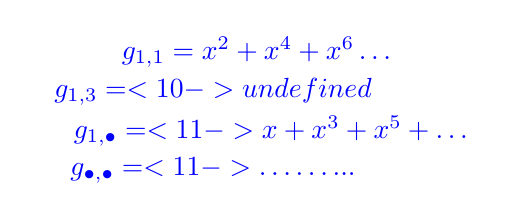
\begin{tikzpicture}
		\node[] (g11) at (1, 1){
%			\resizebox{3.125cm}{!}{
				\ \ \ \ \ \ 
				$\textcolor{blue}{g_{1,1} = \pause x^2 + x^4 + x^6 \ldots}$ 
%			}
		};
			
	
%\onslide<5->
%{	
%		\node[] (g11kopia) at (4, 1){
%			%\resizebox{3.125cm}{!}{
%				\ \ \ \ $g_{1,1} = \textcolor{blue}{g_{1,1} + g_{1,3}(1 + g_{3,3}^+)g_{3,1}}$ 
%			%}
%		};
%}	
	\node[below of=g11, yshift=0.5cm, xshift = -0.2cm] (g13){
%		\resizebox{2.25cm}{!}{
			$\textcolor{blue}{g_{1,3} = \onslide<10->{undefined}}$
%		}
	};
	\node[below of=g13, yshift=0.5cm, xshift = 0.5cm] (g1bullet){
%		\resizebox{2.25cm}{!}{
			%\scalebox{0.6}{
			\ \ \ \	
			$\textcolor{blue}{g_{1,\bullet} = \onslide<11->{x + x^3 + x^5+\ldots}}$
%		}
	};
	\node[below of=g1bullet, yshift=0.5cm, xshift = -0.5cm] (gbulletbullet){
%		\resizebox{2.25cm}{!}{
			%\ \ 
			$\textcolor{blue}{g_{\bullet, \bullet} = \onslide<11->{\ldots \ldots ...}}$
%		}
	};
	\end{tikzpicture}
};
\end{tikzpicture}
\end{frame}
\begin{frame}{Overview ctd. 2}
\begin{tw}['19, Boja{\'n}czyk, S.] The following problem is decidable:\\
	\underline{Input:}
	$$
	\xymatrix{
		\text{treewidth } k	\ar[r] ^{f, g}_{mso} &	\text{treewidth } k	
	}
	$$
	\underline{Question:} Are they equivalent:
	
	$\forall G \in \text{treewidth } k \quad f(G) \sim g(G)$,
	
	$\sim$: \textcolor{blue}{number of length-$n$ walks on $G$ and $H$ are equal, for all $n \geq 0$.}
\end{tw}
\end{frame}
%\fi
\section{xmapsto}
\iffalse%zakomentowanie duzego slajdu
\begin{frame}%the big slide
$G \sim H$ iff \only<1-4>{\textcolor{blue}{number of length-$n$ walks on $G$ and $H$ are equal, for all $n \geq 0$,}}\only<5->{\textcolor{blue}{$g_{\bullet, \bullet} = h_{\bullet, \bullet}$}}
\only<1>%bez greya
{
	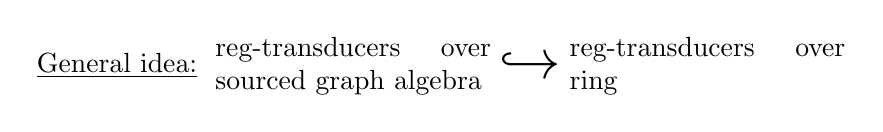
\begin{tikzpicture}
	\node[] (n1){
		\underline{General idea:}
	}; %\sout{
	\node[right of=n1, xshift=2cm] (n2){	
		\parbox{3.5cm}{
			reg-transducers over
			%}
			sourced graph algebra
		}
	};
	\node[right of=n2, xshift = 1.25cm] (n2.5){
		\scalebox{2}{$\hookrightarrow$}
	};
	\node[right of=n2.5, xshift=1.25cm] (n3){
		
		%\sout{
		\parbox{3.5cm}{
			reg-transducers over
			%}
			ring \Zx
		}
	};
	%\node[below of=n2, xshift=-1cm, yshift=-1cm](node def-later){
	%	will be defined later
	%};
	%\draw[-] (node def-later) -- (n2);
	\end{tikzpicture}
}
\onslide<2->%wskakuje grey
{
	
	\begin{tikzpicture}
	\node[] (n1){
		\underline{General idea:}
	}; %\sout{
	\node[right of=n1, xshift=2cm] (n2){	
		\parbox{3.5cm}{
			\textcolor{grey}{reg-transducers over}
			%}
			sourced graph algebra
		}
	};
	\node[right of=n2, xshift = 1.25cm, yshift = -.25cm] (n2.5){
		\scalebox{1.5}{$
			\hookrightarrow
			$}
	};
	\node[right of=n2.5, xshift=1.25cm, yshift = .25cm] (n3){
		
		%\sout{
		\parbox{3.5cm}{
			\textcolor{grey}{reg-transducers over}
			%}
			ring \Zx
		}
	};
	%\only<1-2>{
	%\node[below of=n2, xshift=-1cm, yshift=-1cm](node def-later){
	%	will be defined \only<1>{later}\only<2>{\textcolor{green}{now}}
	%};
	%\draw[-] (node def-later) -- (n2);
	%}
	\end{tikzpicture}
}
%\\
\pause \pause
\\Idea: \pause $G$ $\mapsto$ $g_{\bullet, \bullet} = \sum_{n = 1}^{\infty} a_n x^n$, where $a_n = \#$ walks of length $n$ on $G$. \pause \pause
\begin{tikzpicture}[x = 0.5cm, y = 0.5cm]
\node[](graf1) at (0, 0) {
	\begin{tikzpicture}
	\node[circle] (v1) at (2, 2.5){1};
	\node[circle] (vbull) at (0, 0) {$\bullet$};
	\node[circle] (v3) at (3, 0) {3};
	\draw[-] (v1) -- (vbull) -- (v3);
	\end{tikzpicture}
};

\onslide<10->
{
	\def\szerresizeboxa{1.25cm}
	\node[right of=graf1, xshift = .7cm](ggrafu1){
		\begin{tikzpicture}
		\node[] (g11) at (1, 1){
			\resizebox{\szerresizeboxa}{!}{
				$\textcolor{blue}{g_{1,1} = \onslide<13->{x^2}}$
			}
		};
		\node[below of=g11, yshift=0.5cm] (g13){
			\resizebox{\szerresizeboxa}{!}{
				$\textcolor{blue}{g_{1,3} = \onslide<14->{x^2}}$
			}
		};
		\node[below of=g13, yshift=0.5cm] (g1bullet){
			\resizebox{\szerresizeboxa}{!}{
				$\textcolor{blue}{g_{1,\bullet}\! = \onslide<15->{x}}$
			}
		};
		\node[below of=g1bullet, yshift=0.5cm] (gbulletbullet){
			\resizebox{\szerresizeboxa}{!}{
				$\textcolor{blue}{g_{\bullet,\bullet} = \onslide<16->{0}}$
			}
		};
		\end{tikzpicture}
	};
}
\node[right of= ggrafu1, yshift = -.5cm](przecinek){,
};
\node[right of = przecinek, xshift = 0cm, yshift = .5cm](graf2) {
	\begin{tikzpicture}[x = 0.5cm, y = 0.5cm]
		\node[circle] (w1) at (0,2.5) {1};
		\node[circle] (w3) at (1, 0) {3};
		\draw[-] (w1)--(w3);
	\end{tikzpicture}
};
\onslide<17->
{
	\node[right of=graf2](ggrafu2){
		\begin{tikzpicture}
		\node[] (h11) at (1, 1){
			\resizebox{\szerresizeboxa}{!}{
				$\textcolor{rose}{h_{1,1} = \onslide<18->{0}}$
			}
		};
		\node[below of=h11, yshift=0.5cm] (h13){
			\resizebox{\szerresizeboxa}{!}{
				$\textcolor{rose}{h_{1,3} = \onslide<18->{x}}$
			}
		};
		\node[below of=h13, yshift=0.5cm] (h1bullet){
			\resizebox{\szerresizeboxa}{!}{
				$\textcolor{rose}{h_{1,\bullet} = \onslide<18->{0}}$
			}
		};
		\node[below of=h1bullet, yshift=0.5cm] (hbulletbullet){
			\resizebox{\szerresizeboxa}{!}{
				$\textcolor{rose}{h_{\bullet,\bullet} = \onslide<18->{0}}$
			}
		};
		\end{tikzpicture}
	};
}
%\node[right of=graf2](znak-mapsto){$\xmapsto{join}$
%};
\onslide<7->
{
	\node[right of=ggrafu2, xshift = 2.25cm](graf-join){
	\begin{tikzpicture}
	\node[circle] (v1) at (2, 2.5){1};
	\node[circle] (vbull) at (0, 0) {$\bullet$};
	\node[circle] (v3) at (3, 0) {3};
	\draw[-] (v1) -- (vbull) -- (v3); \draw[-] (v3) -- (v1);
	\end{tikzpicture}
};
}
\onslide<19->
{
	\node[right of=graf-join, xshift = .7cm](ggrafu-join){
		\begin{tikzpicture}
		\node[] (g11) at (1, 1){
			\resizebox{\szerresizeboxa}{!}{
				$g_{1,1} = \onslide<20-29>{\textcolor{black}{x^2}}$
			}
		};
		\node[] (g11) at (1, 1){
		\resizebox{\szerresizeboxa}{!}{
			$g_{1,1} = \onslide<30->{\textcolor{blue}{x^2}}$
			}
		};
		\node[below of=g11, yshift=0.5cm] (g13){
			\resizebox{2.25cm}{!}{
				\ \ \ \ \ $g_{1,3} = \onslide<21-30>{\textcolor{black}{x} + \textcolor{black}{x^2}}$
			}
		};
		\node[below of=g11, yshift=0.5cm] (g13){
			\resizebox{2.25cm}{!}{
				\ \ \ \ \ $g_{1,3} = \onslide<31->{\textcolor{rose}{x} + \textcolor{blue}{x^2}}$
			}
		};
		\node[below of=g13, yshift=0.5cm] (g1bullet){
			\resizebox{\szerresizeboxa}{!}{
				$g_{1,\bullet} = \onslide<22-31>{\textcolor{black}{x}}$
			}
		};
		\node[below of=g13, yshift=0.5cm] (g1bullet){
			\resizebox{\szerresizeboxa}{!}{
				$g_{1,\bullet} = \onslide<32->{\textcolor{blue}{x}}$
			}
		};
		\node[below of=g1bullet, yshift=0.5cm] (gbulletbullet){
			\resizebox{\szerresizeboxa}{!}{
				$g_{\bullet,\bullet} = \onslide<23-29>{0}$
			}
		};
		
		\node[below of=g1bullet, yshift=0.5cm] (gbulletbullet){
			\resizebox{\szerresizeboxa}{!}{
				$g_{\bullet,\bullet} = \onslide<30->{0}$
			}
		};
		\end{tikzpicture}
	};
}
\draw[|->] (ggrafu2) -- (graf-join) node [midway, yshift = 0.25cm] {join};
\only<4>{
%\node[below of=znak-mapsto](znak-mapsto-dol){$\xmapsto{forget}$
};

%
\pause \pause
\def\yshiftnadol{-1cm}
\node[below of=graf1, yshift = \yshiftnadol](graf1-dol){
	\begin{tikzpicture}
	\node[circle] (v1) at (2, 2.5){1};
	\node[circle] (vbull) at (0, 0) {$\bullet$};
	\node[circle] (v3) at (3, 0) {3};
	\draw[-] (v1) -- (vbull) -- (v3);
	\end{tikzpicture}
};
\onslide<24->
{
	\node[right of=graf1-dol, xshift = .7cm](ggrafu1-dol){
		\begin{tikzpicture}
		\node[] (g11) at (1, 1){
			\resizebox{\szerresizeboxa}{!}{
				$\textcolor{blue}{g_{1,1} = x^2}$
			}
		};
		\node[below of=g11, yshift=0.5cm] (g13){
			\resizebox{\szerresizeboxa}{!}{
				$\textcolor{blue}{g_{1,3} = x^2}$
			}
		};
		\node[below of=g13, yshift=0.5cm] (g1bullet){
			\resizebox{\szerresizeboxa}{!}{
				$\textcolor{blue}{g_{1,\bullet} = x}$
			}
		};
		\node[below of=g1bullet, yshift=0.5cm] (gbulletbullet){
			\resizebox{\szerresizeboxa}{!}{
				$\textcolor{blue}{g_{\bullet,\bullet} = 0}$
			}
		};
		\end{tikzpicture}
	};
}
\onslide<9->
{
	\node[below of=graf-join, yshift = \yshiftnadol](graf-forget){
		\begin{tikzpicture}
		\node[circle] (v1) at (2, 2.5){1};
		\node[circle] (vbull) at (0, 0) {$\bullet$};
		\node[circle] (v3) at (3, 0) {$\bullet$};
		\draw[-] (v1) -- (vbull) -- (v3);
		\end{tikzpicture}
	};
}
\onslide<25->
{
	\node[right of=graf-forget, xshift = .7cm](ggrafu-forget){
		\begin{tikzpicture}
\only<25-32>
{
		\node[] (g11) at (1, 1){
			\resizebox{3.125cm}{!}{
				\ \ \ \ $g_{1,1} = x^2 + x^4 + x^6 \ldots$ 
			}
		};
}		
\only<33->
{
		\node[] (g11kopia) at (1, 1){
		\resizebox{3.125cm}{!}{
			\ \ \ \ $g_{1,1} = \textcolor{blue}{g_{1,1} + g_{1,3}(1 + g_{3,3}^+)g_{3,1}}$ 
		}
	};
}
		\node[below of=g11, yshift=0.5cm] (g13){
			\resizebox{2.25cm}{!}{
				$g_{1,3} = \onslide<27->{undefined}$
			}
		};
		\node[below of=g13, yshift=0.5cm] (g1bullet){
			\resizebox{2.25cm}{!}{
			%\scalebox{0.6}{
			\ \	$g_{1,\bullet} = \onslide<28->{\ldots \ldots...}$
			}
		};
		\node[below of=g1bullet, yshift=0.5cm] (gbulletbullet){
			\resizebox{2.25cm}{!}{
				\ \ $g_{\bullet, \bullet} = \onslide<29->{\ldots \ldots ...}$
			}
		};
		\end{tikzpicture}
	};
}
\draw[|->] (ggrafu1-dol) -- (graf-forget) node [midway, yshift = 0.25cm] {forget$_3$};

\end{tikzpicture}


\onslide<10->
{
	$g_{i,j} = \sum_{n=1}^{\infty} a_nx^n, a_n = \#$ of walks from $i$ to $j$ ($i,j \in \allv{G}
	$):
\onslide<11->
{
	\begin{itemize}
		\item positive length,
		\item interiors do not touch sources (walks: $1\bullet 3$ ok, $1 \bullet 3 \bullet \bullet$ not ok)
	\end{itemize}
}
}
\end{frame}

\fi
\begin{frame}{Walk power series are \{join, forget\} - reconstructible.}
Reconstructing series for join and forget:
\begin{align*}
\join(G,H)_{i,j}& = \onslide<2->{g_{i,j} + h_{i,j}} \onslide<3->{\textcolor{grey}{\text{ iff no edge }i-j}}\\
\forget_k(G)_{i,j} &= \onslide<4->{g_{i,j} + g_{i,k}\cdot(1 + g_{k,k}^+)\cdot g_{k,j}}
\end{align*}
\pause \pause \pause
where $f^+ = f + f\cdot f + f\cdot f \cdot f + \ldots \in \Zx$
\\
\pause 
The formulas hold, because:\\
\pause
\begin{itemize}[<+->]
	\item They hold for sets of walks
	\item series = set$[edge:=x]$ -- a formula that respects $+$ and $\cdot$.
\end{itemize}
\pause
\textbf{Now: } how to decide equivalence of register transducers that use $^+$ -- Kleene plus on power series.

\end{frame}

\begin{frame}{$f^+$ -- Kleene plus on power series}
$f^+ = f + f\cdot f + f\cdot f \cdot f + \ldots \in \Zx$ (defined iff $f(0) = 0$).\\
We have $f^+ = f+ f\cdot f^+$, hence\\
$$
	f^+ = \frac{f}{1-f}.
$$
\pause
\begin{enumerate}[<+->]
	\item Make computations possible (registers store fractions of polynomials)
	\item \only<3>{\textcolor{red}{Uses division}}\only<4->{\textcolor{green}{Uses division}}.
\end{enumerate}
\onslide<4->
{
	\begin{tw}['19, Boja{\'n}czyk, S.]
		Equivalence is decidable for polynomial automata with \textcolor{green}{division} (over any computable ring without zero divisors).
	\end{tw}
}
\end{frame}
\begin{frame}{Polynomial automata with division}
\begin{lm}
	For any polynomial automaton with division $A: t \mapsto A(t)$ there is a polynomial automaton $B: t \mapsto (B_1(t), B_2(t))$ which ''simulates'' $A$ in the following sense:
	$$
		A(t) = \frac{B_1(t)}{B_2(t)}.
	$$	
\end{lm}
\pause
\underline{Proof:}
\pause
\\
	Like projective line: $\frac{x_1}{x_2} \lra (x_1, x_2)$.\\
	$\left(\frac{x_1}{x_2}\right)^+ = \frac{\frac{x_1}{x_2}}{1-\frac{x_1}{x_2}} = \frac{x_1}{x_2-x_1}$.\\
	So we define $(x_1, x_2)^+ = (x_1, x_2 - x_1)$. Similarly $+, \cdot: K\times K \ra K\times K$.	
\end{frame}
\begin{frame}{Final remarks, Future work}
\begin{itemize}[<+->]
	\item Rephrasing: We are looking for a graph polynomial and its extension to sourced graphs, that is:
	\begin{itemize}
		\item \underline{complete invariant} on class ''treewidth $k$ graphs'',
		\item \underline{reconstructible} with join and forget operations of sourced graphs.
	\end{itemize}
\onslide<4->{ open even for $k=1$, i.e. unrooted trees. solved for rooted (unordered) trees ['18, Boiret, Pi{\'o}rkowski, S.].}\pause
	\item \underline{Known polynomials}.
	 ['73, Schwenk] Characteristic polynomial and Tutte polynomial fail badly to characterize even trees!
	\item investigate \underline{branching walks} -- equivalent to fractional isomorphism ['18, Dell et al.]
	\item restrict the class of outputted graphs, e.g. to labelled cycles.
\end{itemize}
\end{frame}
\end{document}
\begin{frame}{Slajd przykładowy}

\begin{tikzpicture}
\node (nodek 1) {asd};
\node [below of= nodek 1, left of=nodek 1, yshift=-15pt] (etykieta 1) {\textcolor{grey}{later}};
\draw[-] (nodek 1) -- (etykieta 1);
\end{tikzpicture}
%R.A. over s.g.a $\hookrightarrow $ R.A. over \ringint.
\end{frame}